%%
%% Copyright 2019-2024 Elsevier Ltd
%%
%% This file is part of the 'CAS Bundle'.
%% --------------------------------------
%%
%% It may be distributed under the conditions of the LaTeX Project Public
%% License, either version 1.3c of this license or (at your option) any
%% later version.  The latest version of this license is in
%%    http://www.latex-project.org/lppl.txt
%% and version 1.3c or later is part of all distributions of LaTeX
%% version 1999/12/01 or later.
%%
%% The list of all files belonging to the 'CAS Bundle' is
%% given in the file `manifest.txt'.
%%
%% Template article for cas-dc documentclass for
%% double column output.

% Course brief: 11 pt body text, Times New Roman, 12/14 pt headings (class default).
\documentclass[a4paper,fleqn,11pt]{cas-dc}
\usepackage[numbers]{natbib}
\usepackage{placeins}
% Times text: newtxtext on Overleaf, URW Times (mathptmx) where newtx is not installed.
\IfFileExists{newtxtext.sty}{\usepackage{newtxtext}}{\renewcommand{\rmdefault}{ptm}}
\usepackage{tikz}
\usetikzlibrary{arrows.meta,positioning,fit,backgrounds,calc}
\usepackage{algorithm}
\usepackage{algpseudocode}
\usepackage{array}
\newcolumntype{L}[1]{>{\raggedright\arraybackslash}p{#1}}
\emergencystretch=1em

% If the frontmatter runs over more than one page
% use the longmktitle option.

%\documentclass[a4paper,fleqn,longmktitle]{cas-dc}

%\usepackage[authoryear]{natbib}

%%%Author macros
\def\tsc#1{\csdef{#1}{\textsc{\lowercase{#1}}\xspace}}
\tsc{WGM}
\tsc{QE}
%%%

% Marks used in the comparison table
\newcommand{\cmyes}{$\checkmark$}
\newcommand{\cmno}{$\times$}
\newcommand{\cmpart}{$\circ$}

\begin{document}
\let\WriteBookmarks\relax
\let\printorcid\relax
\ExplSyntaxOn
\cs_set:Npn \__first_footerline: {\small\sffamily Khan~and~Khalid:~\itshape Course~CEP~research~report}
\ExplSyntaxOff
\def\floatpagepagefraction{1}
\def\textpagefraction{.001}

% Short title
\shorttitle{SLO-Aware Chaos Engineering for Cloud-Native Applications}

% Short author
\shortauthors{Khan and Khalid}

% Main title of the paper
\title [mode = title]{SLO-Aware Chaos Engineering for Cloud-Native Applications}

\author[1]{Muhammad Awwab Khan}%[<options>]

% Corresponding author indication
\cormark[1]

% Footnote of the first author
\fnmark[1]

% Email id of the first author
\ead{khan4600966@cloud.neduet.edu.pk}

% Address/affiliation
\affiliation[1]{organization={Department of Software Engineering, NED University of Engineering and Technology},
            city={Karachi},
            state={Sindh},
            country={Pakistan}}

\author[2]{Muhammad Abyaz Khalid}%[]

% Footnote of the second author
\fnmark[2]

% Email id of the second author
\ead{khalid4600054@cloud.neduet.edu.pk}

% Address/affiliation
\affiliation[2]{organization={Department of Software Engineering, NED University of Engineering and Technology},
            city={Karachi},
            state={Sindh},
            country={Pakistan}}

% Corresponding author text
\cortext[1]{Corresponding author}

% Footnote text
\fntext[1]{Roll Number: SE-23051}
\fntext[2]{Roll Number: SE-23053}

% Here goes the abstract
\begin{abstract}
Chaos experiments cause failures on purpose, so they use up part of the error budget that a service level objective (SLO) allows. We study how to keep an experiment within the share of that budget an operator gives it, while still injecting enough faults to be useful. We built separate request-count ledgers for an availability SLO (99\%) and a latency SLO (95\% of requests within 500\,ms), estimated the loss caused by the experiment by comparing it with a matched control stack, and compared four ways of choosing the percentage of requests that receive an injected HTTP delay or abort: a static rate, a threshold stop, a pilot-calibrated open-loop rate and a closed-loop feedback controller. All four share a safety reserve, an independent watchdog that removes expired faults, and telemetry checks that stop injection when data is missing or stale. On a single-node Kubernetes/Istio cluster we ran 80 policy comparisons, 10 no-fault controls and 20 background-error ablations, each with a 120\,s warmup, a 300\,s fault window and 120\,s recovery. No run exceeded its allocation, and all ten controls consumed zero budget. Closed-loop control removed the 4.6--21.6 request overshoot that static injection made past the safety guard, but it injected fewer faults: for aborts, its exposure (the injected fault fraction integrated over time) was about nine fraction-seconds lower than that of open-loop injection. The run traces show that burn-rate gates held abort intensity near 2\%. A budget-paced policy, designed after these results and tested in 20 separate runs, spent 98--100\% of the usable allocation, came within 0.62 fraction-seconds of static exposure and reduced mean guard overshoot to 0.8--1.6 requests, again with no run exceeding its allocation. The best policy therefore depends on the workload and on how much safety margin the operator wants.
\end{abstract}

% Keywords
% Each keyword is seperated by \sep
\begin{keywords}
Chaos engineering \sep Service level objectives \sep Error budget \sep Fault injection \sep Kubernetes \sep Istio \sep Site reliability engineering
\end{keywords}

\maketitle

%% ===========================================================================
\section{Introduction}\label{sec:intro}
%% ===========================================================================

Cloud native applications are built from many loosely coupled microservices that run in containers on platforms such as Kubernetes \citep{kratzke2017understanding,burns2016borg}. This design supports independent deployment and elastic scaling, but it also creates deep chains of network dependencies. Failures propagate across these dependencies, and the many service interactions make them harder to detect and to localize \citep{soldani2023anomaly}. Rare slow responses in individual services dominate the tail latency that users experience \citep{dean2013tail}. Distributed concurrency bugs, triggered by badly timed interactions between nodes, cause data loss and service outages \citep{lu2022cloudraid}, and gray failures leave a component running but degraded, which makes them hard to catch with static alarms \citep{ye2026a3sm}.

Chaos engineering addresses these problems by injecting controlled faults into a running system and checking whether its steady state holds \citep{basiri2016chaos}. It is now widely applied to microservice systems and supported by many tools \citep{owotogbe2026chaos,esen2026chaos}. In parallel, site reliability engineering defines reliability through service level objectives (SLOs). In this paper, the error budget is the gap between an SLO target and perfect reliability over a time window, and the burn rate is the rate at which this budget is consumed relative to the rate that would exhaust it exactly at the end of the window. Recent work treats the error budget as a dynamic resource that a controller can consume in a controlled way to reach other objectives \citep{souza2026bahya}.

A chaos experiment uses up part of the error budget while it tests a service. Injecting too many faults can exhaust the allowed share, and injecting too few gives little evidence. Delay experiments under different loads illustrate the sensitivity of service outcomes to fault settings \citep{ahmad2024exploring}. Netflix's ChAP already uses baseline and canary clusters, request-level faults and automated safety mechanisms \citep{basiri2019automating}. Error-budget-aware placement and SLO-aware timeout controllers provide related control ideas \citep{souza2026bahya,hanada2025slo}. Our contribution is an experimental evaluation that combines attributed loss accounting, separate SLO constraints and fault-intensity feedback. Our literature search was not exhaustive, so we do not claim that no similar work exists.

The main objective of this study is to develop and evaluate a chaos engineering framework whose fault intensity is governed by the error budget that the experiment consumes. Specifically, the study aims to (i) keep the budget consumed by an experiment within an allocation set by the operator, (ii) separate experiment induced consumption from organic consumption, and (iii) support both availability and tail latency SLOs.

The implementation contains a Budget Accountant, an Attribution Engine, an Intensity Controller and an empirical Budget Oracle. A small instrumented frontend and dependency run in separate treatment and control stacks on Kubernetes with Istio and Prometheus. We compare static intensity, threshold stop, pilot-calibrated open-loop injection and budget-feedback closed-loop control, and we evaluate a budget-paced variant of the controller in a separate follow-up. We did not use Online Boutique or Chaos Mesh; both are left for future work.

The main contributions of this work are:
\begin{itemize}
\item an explicit request-count formulation of separate SLO allocations and cleanup reserves;
\item an implementation of signed excess-loss estimation with conditional, sequential background credit;
\item a reproducible Kubernetes controller, independent watchdog, and evidence protocol that distinguishes operational checks from comparative research results;
\item a trace-level diagnosis of why burn-rate gates under-use an experiment allocation, with a budget-paced alternative evaluated separately.
\end{itemize}

The rest of this paper is organized as follows. Section~\ref{sec:lit} reviews related work and Section~\ref{sec:compare} compares the closest approaches and our policies. Section~\ref{sec:method} presents the failure model, architecture, accounting and control algorithms. Section~\ref{sec:impl} describes the experimental setup and test scenarios, Section~\ref{sec:results} reports results, Section~\ref{sec:discussion} discusses insights, validity threats and professional considerations, and Section~\ref{sec:conclusion} concludes.

%% ===========================================================================
\section{Related Work}\label{sec:lit}
%% ===========================================================================

This section reviews chaos engineering and fault injection for microservices, adaptive and SLO-aware control in cloud systems, and the use of error budgets as a control resource, and then states the research gap.

\subsection{Chaos engineering and fault injection}\label{sec:lit:ce}

Several studies show why cloud native systems need resilience testing. A review of microservice adoption reports new difficulties in testing and monitoring the many interactions between services \citep{soldani2018pains}, and a survey of anomaly detection and root cause analysis shows that failures propagate across services, which makes their causes hard to identify \citep{soldani2023anomaly}. Distributed concurrency bugs are triggered by unexpected message orderings between nodes and are hard to find \citep{lu2022cloudraid}, and gray failures degrade a component without stopping it \citep{ye2026a3sm}.

\citet{basiri2016chaos} defined chaos engineering through four principles: a hypothesis about steady state behavior, real world events, experiments in production, and continuous automation. Their method compares a control group with an experimental group and treats a difference in the steady state metric as a weakness. A multivocal literature review derives a unified definition of chaos engineering and a taxonomy of chaos engineering platforms \citep{owotogbe2026chaos}, and a systematic review examines fault-injection tools in microservice systems \citep{esen2026chaos}. A retrospective of ten years of chaos engineering names large language model assisted test automation, hybrid testing frameworks and integration with compliance and governance workflows as next directions \citep{owotogbe2026ten}.

Research on fault injection has made experiments more systematic. A systematic review of fault injection testing for microservice systems summarizes a general framework of five components, each of which represents a design decision that the tester must determine \citep{yu2025systematic}. FBFI iteratively infers and injects fault-tolerance bottlenecks to test redundant components \citep{wu2023enhancing}, and MicroFI restricts faults to selected requests and prioritizes high impact faults \citep{chen2024microfi}. Other work makes injected faults more realistic by deriving them from system call errors observed in production \citep{zhang2022maximizing}, analyzes exception handling in the JVM through chaos experiments \citep{zhang2021chaos}, and provides a configurable chaos platform for hybrid cloud systems \citep{camacho2022chaos}. An empirical study injects delays of different lengths into cloud native applications under different user loads and observes that availability problems appear suddenly at a particular delay \citep{ahmad2024exploring}. We reviewed these studies through their published descriptions, not their full algorithms, so we cannot say for certain that none of them controls fault intensity with an error budget.

\subsection{Adaptive and SLO-aware control}\label{sec:lit:adaptive}

Recent work makes cloud systems react to faults and SLOs in a closed loop. The reported UNFRAGILE latency case study uses progressively injected latency and adapts application fault tolerance, including asynchronous requests, timeouts and concurrency limits \citep{botros2024towards}. A load-adaptive timeout mechanism adjusts timeout values in microservices to keep failure rate and latency SLOs, and it is evaluated on Online Boutique \citep{hanada2025slo}. A3SM uses hierarchical reinforcement learning to decide when and where to migrate workloads under gray failures, and it attributes anomaly impact to tasks, nodes and groups before it acts \citep{ye2026a3sm}. These systems adjust timeouts, workload placement or fault tolerance. Our prototype adjusts the percentage of requests that receive a fault, and that difference alone does not make it novel.

\subsection{Error budgets as a control resource}\label{sec:lit:slo}

SLOs, error budgets and burn rates are the basis of reliability management in site reliability engineering practice. In research, BAHYA treats the SLA error budget of an application as a dynamic, manageable resource: a deep reinforcement learning agent consumes a controlled portion of the budget to trade latency, energy efficiency and resilience in application placement, and it is evaluated in simulation \citep{souza2026bahya}. BAHYA shows that an error budget can drive a closed-loop controller, although it changes application placement while our controller changes the fault percentage.

\citet{bertsch2025chaos} describes a patent in which chaos injection rates are limited by SLO budgets and burn rates, the injector is updated repeatedly, and faults are applied as Envoy HTTP faults. This already covers the general idea of SLO-governed fault rates, so our contribution is an empirical evaluation of particular accounting and control choices.

\subsection{Research gap}\label{sec:lit:gap}

Table~\ref{tbl:compare} shows where our study sits among these approaches. We ask whether feedback changes allocation overshoot and useful exposure (RQ1), whether signed attribution estimates improve on total-failure accounting under known background errors (RQ2), what trade-off exists between safety and exposure (RQ3), and how telemetry lag, load and multiple SLO constraints affect controller behavior (RQ4). RQ1--RQ3 are evaluated on the cluster; RQ4 is addressed only through unit tests and the load factor, because the planned single-SLO and delayed-telemetry cluster ablations were not collected. We report negative and inconclusive comparisons as results.

%% ===========================================================================
\section{Comparative Analysis}\label{sec:compare}
%% ===========================================================================

Table~\ref{tbl:compare} compares the closest reviewed approaches along four dimensions: what the mechanism actuates, which signal governs it, whether a control cohort separates experiment effects from organic behavior, and how it was evaluated. Each entry summarizes the description in Section~\ref{sec:lit}. A cross or circle means we did not find the feature in that description; the source may still have it.

\begin{table*}[width=\textwidth,cols=5,pos=t]
\caption{Comparison of the closest reviewed approaches with this study, based on the descriptions in Section~\ref{sec:lit}.}\label{tbl:compare}
\small
\begin{tabular*}{\tblwidth}{@{\extracolsep{\fill}}L{2.6cm}L{3.2cm}L{3.6cm}L{2.6cm}L{3.8cm}@{}}
\toprule
Source & Actuator & Governing signal & Control cohort & Evaluation \\
\midrule
\citet{basiri2016chaos} & Real-world fault events & Steady-state hypothesis & \cmyes{} control vs.\ experimental group & Production practice \\
\citet{basiri2019automating} & Request-level faults & Automated safety mechanisms & \cmyes{} baseline and canary clusters & Production platform \\
\citet{ahmad2024exploring} & Delay length under load & None (fixed settings) & \cmno & Cloud-native applications \\
\citet{botros2024towards} & Progressive latency; adapts fault tolerance & \cmpart{} not described here & \cmpart{} not described here & Latency case study \\
\citet{hanada2025slo} & Timeout values & Failure-rate and latency SLOs & \cmno & Online Boutique \\
\citet{souza2026bahya} & Application placement & SLA error budget (DRL) & \cmno & Simulation \\
\citet{bertsch2025chaos} & Injection rate & SLO budget and burn & \cmpart{} not described here & Patent description \\
\textbf{This study} & Request-fault percentage (Istio) & Two count-based SLO ledgers; allocation, reserve and pace & \cmyes{} matched stacks & Kubernetes/Istio lab: 110 study runs, 20 follow-up runs \\
\bottomrule
\end{tabular*}
\end{table*}

The table shows two things. SLO-governed fault rates \citep{bertsch2025chaos} and matched cohorts \citep{basiri2019automating} already exist, so we claim only an empirical evaluation of one accounting and control combination. Also, most adaptive work changes the application (its timeouts, placement or fault tolerance) to protect SLOs, while we change the experiment itself and treat the SLO budget as its limit.

Table~\ref{tbl:policies} compares the five fault-intensity policies that we implemented. All share the same allocation, reserve, maximum intensity (10\%), emergency guards and watchdog, so they differ only in how they choose the intensity.

\begin{table*}[width=\textwidth,cols=4,pos=t]
\caption{Fault-intensity policies compared in this study. $A_j$: allocation; $D_j$: debit; $R$: reserve; $u$: fault percentage.}\label{tbl:policies}
\small
\begin{tabular*}{\tblwidth}{@{\extracolsep{\fill}}L{2.2cm}L{5.4cm}L{3.8cm}L{4.4cm}@{}}
\toprule
Policy & Rule & Strength & Weakness \\
\midrule
Static & Fixed $u=10\%$ until a common guard stops it & Maximum exposure; no tuning & Runs into the guard; overshoot equals guard reaction lag \\
Threshold & Static, but stops when interval burn $\geq 2$ & Very low consumption & With $q=1\%$, any abort above 2\% stops on the first tick \\
Open-loop & Fixed $u=(A_j-R)/(N_F\,c)$ from a pilot cost $c$ & Spends the allocation with no feedback & Depends on an accurate pilot; cannot react to drift \\
Closed-loop & AIMD: halve if projected risk $>1$ or short and long burn $>2$; add 0.5\,pp if risk $<0.5$ and burn $<1$ & Reacts to observed loss & Burn gates are absolute, so they cap abort intensity near 2\% \\
Paced (follow-up) & AIMD on consumption relative to $(A_j-D_j-R)/t_{\text{rem}}$ & Gates scale with the remaining allocation & Pushes intensity up near the end of the window; post-result design \\
\bottomrule
\end{tabular*}
\end{table*}

\FloatBarrier

%% ===========================================================================
\section{Methodology}\label{sec:method}
%% ===========================================================================

\subsection{Failure model and requirements}\label{sec:threat}
The risk we address is the chaos experiment itself. A fault injector that runs on live traffic can (T1) exhaust the error budget and harm users, (T2) leave a fault active after its controller crashes, (T3) keep injecting while telemetry is stale or missing, so damage goes unseen, (T4) blame organic failures on the experiment or hide experiment damage behind them, and (T5) target the wrong service or namespace. Table~\ref{tbl:threats} maps each risk to the mechanism that addresses it and to the evidence we collected. The functional requirements are: account each SLO in request counts; keep consumption within a frozen allocation; stop safely whenever the data is in doubt; and keep auditable evidence of every decision.

\begin{table}[width=.95\linewidth,cols=3,pos=t]
\caption{Failure model: risks, mechanisms and evidence.}\label{tbl:threats}
\footnotesize
\begin{tabular*}{\tblwidth}{@{}L{1.6cm}L{3.0cm}L{2.4cm}@{}}
\toprule
Risk & Mechanism & Evidence \\
\midrule
T1 budget exhaustion & Frozen allocation, reserve $R$, common guard, policy & Guard overshoot (Sec.~\ref{sec:results}) \\
T2 stuck fault & 6\,s fault lease; independent watchdog; cleanup readback & Kill test, expiry test \\
T3 blind injection & Freshness, gap, epoch and traffic gates; fail closed & Host-suspend incident \\
T4 misattribution & Matched control; signed estimate; conditional credit & Background ablation \\
T5 wrong target & Namespace marked disposable; route to one host; named-resource Role & Treatment-only check \\
\bottomrule
\end{tabular*}
\end{table}

\subsection{Architecture}
Figure~\ref{fig:arch} shows the system. A host-side k6 generator sends matched constant-arrival traffic to the control and treatment frontends and writes one raw outcome per request. The Budget Accountant reads these outcomes, the Attribution Engine compares cohorts, and the Intensity Controller selects a fault percentage that the Istio adapter writes to a single VirtualService with an expiry annotation. The Envoy sidecar applies the fault only to calls to the treatment dependency. A separately started watchdog renews a heartbeat and removes any fault whose lease has expired. Every observation, decision and ledger state is appended to an event log and sealed with checksums.

\begin{figure*}[t]
\centering
\resizebox{\textwidth}{!}{%
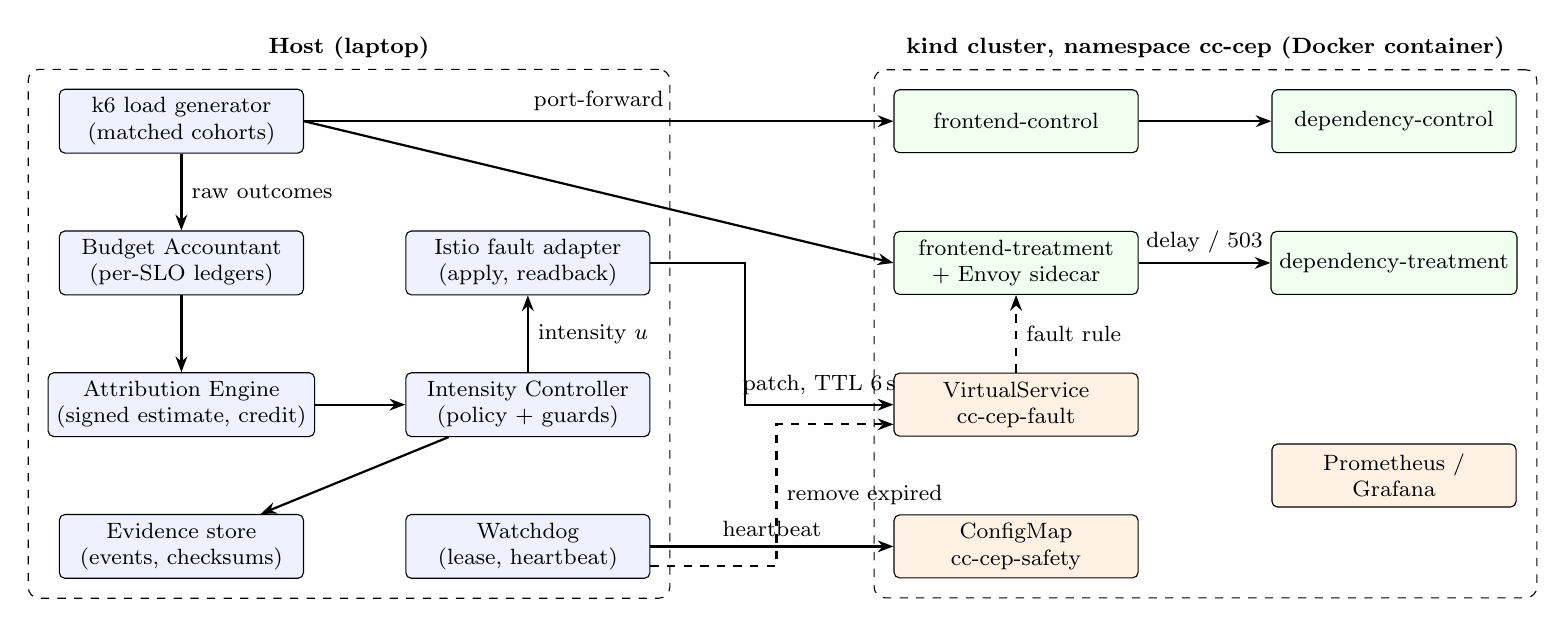
\begin{tikzpicture}[
  font=\footnotesize,
  box/.style={draw, rounded corners=2pt, align=center, minimum height=8mm, minimum width=31mm, inner sep=3pt},
  comp/.style={box, fill=blue!6},
  pod/.style={box, fill=green!6},
  res/.style={box, fill=orange!10},
  arr/.style={-{Stealth[length=2mm]}, thick},
  fltdash/.style={-{Stealth[length=2mm]}, thick, dashed}]
  % Host side
  \node[comp] (k6) at (0,0) {k6 load generator\\(matched cohorts)};
  \node[comp] (acc) at (0,-1.8) {Budget Accountant\\(per-SLO ledgers)};
  \node[comp] (att) at (0,-3.6) {Attribution Engine\\(signed estimate, credit)};
  \node[comp] (ev) at (0,-5.4) {Evidence store\\(events, checksums)};
  \node[comp] (ad) at (4.4,-1.8) {Istio fault adapter\\(apply, readback)};
  \node[comp] (ctl) at (4.4,-3.6) {Intensity Controller\\(policy + guards)};
  \node[comp] (wd) at (4.4,-5.4) {Watchdog\\(lease, heartbeat)};
  \begin{scope}[on background layer]
    \node[draw, dashed, rounded corners, fit=(k6)(acc)(att)(ctl)(wd)(ev)(ad), inner sep=7pt, label={[font=\footnotesize\bfseries]above:Host (laptop)}] {};
  \end{scope}
  % Cluster side
  \node[pod] (fc) at (10.6,0) {frontend-control};
  \node[pod] (dc) at (15.4,0) {dependency-control};
  \node[pod] (ft) at (10.6,-1.8) {frontend-treatment\\+ Envoy sidecar};
  \node[pod] (dt) at (15.4,-1.8) {dependency-treatment};
  \node[res] (vs) at (10.6,-3.6) {VirtualService\\cc-cep-fault};
  \node[res] (cm) at (10.6,-5.4) {ConfigMap\\cc-cep-safety};
  \node[res] (pm) at (15.4,-4.5) {Prometheus /\\Grafana};
  \begin{scope}[on background layer]
    \node[draw, dashed, rounded corners, fit=(fc)(dc)(ft)(dt)(vs)(cm)(pm), inner sep=7pt, label={[font=\footnotesize\bfseries]above:kind cluster, namespace cc-cep (Docker container)}] {};
  \end{scope}
  \draw[arr] (k6.east) -- node[above, pos=0.5] {port-forward} (fc.west);
  \draw[arr] (k6.east) -- (ft.west);
  \draw[arr] (fc) -- (dc);
  \draw[arr] (ft) -- node[above] {delay / 503} (dt);
  \draw[arr] (k6) -- node[right] {raw outcomes} (acc);
  \draw[arr] (acc) -- (att);
  \draw[arr] (att) -- (ctl);
  \draw[arr] (ctl) -- node[right] {intensity $u$} (ad);
  \draw[arr] (ad.east) -- ++(1.2,0) |- node[pos=0.75, above] {patch, TTL 6\,s} (vs.west);
  \draw[fltdash] (vs) -- node[right] {fault rule} (ft);
  \draw[arr] (wd.east) -- node[above] {heartbeat} (cm.west);
  \draw[fltdash] (wd.east) ++(0,-0.25) -- ++(1.6,0) |- node[pos=0.25, right] {remove expired} ($(vs.west)+(0,-0.25)$);
  \draw[arr] (ctl) -- (ev);
\end{tikzpicture}}
\caption{System architecture. Solid arrows carry data or commands; dashed arrows show the fault rule and the watchdog's removal path. Prometheus and Grafana provide supporting telemetry only; ledgers use raw client outcomes.}\label{fig:arch}
\end{figure*}

\subsection{Request eligibility and independent ledgers}
Every completed client request to the business endpoint is eligible. HTTP failures and client timeouts are availability-bad events. A request is latency-bad if it exceeds 500\,ms or fails, so one request can be bad for both SLOs. We never add the ledgers together. With target $s_j$, allowed bad fraction $q_j=1-s_j$, expected reservation traffic $N_H$ and allocation fraction $f_j$, admission freezes $A_j=f_jq_jN_H$. This experiment allocation stays fixed and is separate from the service's remaining balance in the observed window, $q_jN-B_j$. In the study we set $A_j=R+H$ with usable headroom $H=\lceil 0.5\cdot 0.1\cdot 300\,r\rceil$ at load $r$, chose $N_H=\lceil 2A/0.01\rceil+1$, and derived $f_j$ so both SLOs receive the same number of bad requests ($f\approx0.5$ for availability, $0.1$ for latency). The allocation is therefore a choice we made for the laboratory; we did not derive it from a production SLO window.

The supported reserve is $R=\lambda_{\max}L$, where $\lambda_{\max}$ is the traffic cap and $L$ includes observation delay, fault lease, request timeout and API/removal margin. Admission rejects $A_j\leq R$. Remaining usable allocation is $A_j-D_j-R$, where $D_j$ is the enforcement debit. The reservation traffic $N_H$ only sizes the laboratory budget. A 300\,s experiment does not show that the service would meet its SLO over that longer horizon.

\subsection{Attribution and uncertainty}
For aligned interval $k$, the signed excess estimate is
\begin{equation}
 \widehat E_{jk}=B^T_{jk}-N^T_k B^C_{jk}/N^C_k.
\end{equation}
We retain negative estimates for analysis. The default debit is the cumulative observed treatment bad count, so uncertainty never creates a realized event and zero bad requests consume zero budget.

A declared stationary, independent Bernoulli background model permits conservative credit. Invert the beta-mixture likelihood-ratio confidence sequence for control outcomes \citep{howard2021timeuniform} to obtain a lower background-rate bound $p^-_n$. With a separately allocated error probability $\delta$, define
\begin{equation}
 L_B(n)=\max\{0,np^-_n-\sqrt{2np^-_n\log(\pi^2n^2/(6\delta))}\}.
\end{equation}
A Chernoff bound and a union bound over request counts motivate this lower bound on realized counterfactual background events. Error probability is split between the confidence sequence and the count bound, and across SLOs. The cumulative debit uses
\begin{equation}
 D_j(k)=\max\{D_j(k-1),\,0,\,B^T_j(k)-L_B(N^T(k))\}.
\end{equation}
Thus $0\leq D_j\leq B^T_j$ and zero observed bad events imply zero debit. Credit requires independent, identical, stationary organic outcomes and a monotone fault model under which injection cannot remove organic bad events. Shared failures, drift or contamination invalidate that interpretation. Without the declared model, the controller grants no background credit. The confidence sequence and the count bound are established tools; we apply them and do not propose a new causal estimator.

\subsection{Control algorithm}
Algorithm~\ref{alg:tick} shows one control tick, executed every two seconds. Guards run first and are identical for every policy. The closed-loop policy uses SRE burn rate $\beta_j=(B_j/N)/q_j$ over 5\,s and 30\,s windows together with the projected risk
\begin{equation}
\rho_j=\frac{D_j/t_{\text{el}}\cdot t_{\text{rem}}}{A_j-D_j-R},
\end{equation}
where $t_{\text{el}}$ and $t_{\text{rem}}$ are elapsed and remaining fault-window time. The paced follow-up policy replaces burn rate with pace $\pi_j=r_j/[(A_j-D_j-R)/t_{\text{rem}}]$, the observed bad-request rate $r_j$ divided by the rate that would spend the remaining usable allocation exactly on time.

\begin{algorithm}[t]
\caption{One control tick}\label{alg:tick}
\footnotesize
\begin{algorithmic}[1]
\Require snapshot $S_k$, previous $S_{k-1}$, ledgers $L_j$, intensity $u$
\If{$S_k$ invalid (stale, gap, reset, low traffic or over cap)}
  \State \Return \textsc{Stop}(fail closed)
\EndIf
\For{each SLO $j$}
  \State update $B^T_j$, $\widehat E_j$ and $D_j$ (Eqs.~1--3)
  \If{$D_j+R\geq A_j$ \textbf{or} $\beta_j\geq20$}
    \State \Return \textsc{Stop}(guard)
  \EndIf
\EndFor
\If{fault window elapsed}
  \State \Return \textsc{Stop}(duration)
\EndIf
\If{policy = threshold \textbf{and} $\max_j\beta_j\geq2$}
  \State \Return \textsc{Stop}(policy)
\EndIf
\If{cooldown of 2\,s has passed}
  \If{policy = closed-loop}
    \If{$\max_j\rho_j>1$ \textbf{or} short and long $\beta>2$}
      \State $u\gets u/2$
    \ElsIf{$\max_j\rho_j<0.5$ \textbf{and} short and long $\beta<1$}
      \State $u\gets\min(u_{\max},u+0.005)$
    \EndIf
  \ElsIf{policy = paced}
    \If{$\exists j:\rho_j>1$ \textbf{or} ($\pi^{5s}_j>2$ \textbf{and} $\pi^{30s}_j>1$)}
      \State $u\gets u/2$
    \ElsIf{$\forall j:\rho_j<0.9$, $\pi^{5s}_j<1$, $\pi^{30s}_j<1$}
      \State $u\gets\min(u_{\max},u+0.005)$
    \EndIf
  \EndIf
\EndIf
\State write $u$ with a 6\,s lease; append event; \Return $u$
\end{algorithmic}
\end{algorithm}

Static injection fixes the maximum percentage. Threshold stop also reacts to interval burn. The open-loop policy uses an independently measured cost and the usable allocation divided by expected fault-window traffic. Cooldown and distinct increase/decrease thresholds reduce rapid oscillation.

\subsection{Run lifecycle and safety}
Each run follows the state machine in Figure~\ref{fig:fsm}. All policies share allocation and total-health guards, fresh-data and minimum-traffic gates, a traffic cap, finite fault duration and an emergency stop file. Freshness uses the decision clock after API inspection; a second client-expiry check precedes each fault write. The external watchdog maintains a heartbeat in a separate ConfigMap so it cannot rewrite active fault routing, and it removes faults whose lease has expired. Cleanup retries require API readback; exhausted cleanup sets a sticky failed flag, even if a later removal succeeds. Counts observed through cleanup and recovery remain in the ledger. Sending a stop request does not prove that the fault is gone, and because the Kubernetes API can fail, the system cannot guarantee safety unconditionally.

\begin{figure}[t]
\centering
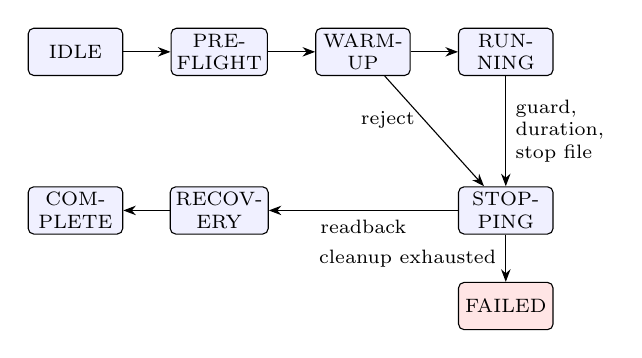
\begin{tikzpicture}[font=\scriptsize, node distance=7mm and 6mm,
  st/.style={draw, rounded corners=2pt, fill=blue!6, minimum width=12mm, minimum height=6mm, align=center, inner sep=2pt},
  arr/.style={-{Stealth[length=1.6mm]}}]
  \node[st] (idle) {IDLE};
  \node[st, right=of idle] (pre) {PRE-\\FLIGHT};
  \node[st, right=of pre] (warm) {WARM-\\UP};
  \node[st, right=of warm] (run) {RUN-\\NING};
  \node[st, below=14mm of run] (stop) {STOP-\\PING};
  \node[st, below=14mm of pre] (rec) {RECOV-\\ERY};
  \node[st, below=14mm of idle] (done) {COM-\\PLETE};
  \node[st, below=6mm of stop, fill=red!10] (fail) {FAILED};
  \draw[arr] (idle) -- (pre);
  \draw[arr] (pre) -- (warm);
  \draw[arr] (warm) -- (run);
  \draw[arr] (run) -- node[right, align=left]{guard,\\duration,\\stop file} (stop);
  \draw[arr] (warm) -- node[left, pos=0.4]{reject} (stop);
  \draw[arr] (stop) -- node[below]{readback} (rec);
  \draw[arr] (rec) -- (done);
  \draw[arr] (stop) -- node[left]{cleanup exhausted} (fail);
\end{tikzpicture}
\caption{Controller run lifecycle. Any failure passes through STOPPING, where fault removal must be read back before RECOVERY.}\label{fig:fsm}
\end{figure}

\subsection{Data structures and design patterns}
Table~\ref{tbl:design} lists the main data structures and design patterns in the implementation (Python 3.12, about 3,700 lines in \texttt{src/}, with 66 unit and integration tests).

\begin{table}[width=.95\linewidth,cols=2,pos=t]
\caption{Data structures and design patterns.}\label{tbl:design}
\footnotesize
\begin{tabular*}{\tblwidth}{@{}L{2.2cm}L{5.1cm}@{}}
\toprule
Element & Role \\
\midrule
\texttt{Counts} & Immutable cumulative counters (total, availability-bad, latency-bad); validates latency-bad $\geq$ availability-bad and detects counter resets \\
\texttt{Snapshot} & Timestamped pair of control and treatment counts with a counter epoch \\
\texttt{Ledger} & Per-SLO allocation, signed estimate, enforced high-water debit and background bound \\
\texttt{Config} & Frozen, validated parameter set; rejects non-finite or inconsistent values \\
State machine & Explicit run lifecycle (Fig.~\ref{fig:fsm}) \\
Strategy & Interchangeable intensity policies behind one tick interface \\
Fail-closed guard & Any doubt about data stops injection rather than continuing \\
Lease + dead-man's switch & Fault expiry annotation and independent watchdog \\
Idempotent reconcile & Clear, then read back, with bounded retries \\
Event sourcing & Append-only event log; replay rebuilds ledgers and reconciles raw counts \\
Content addressing & SHA-256 sealing of every run directory and archive \\
Single-writer lock & Host file lock prevents two controllers on one cluster \\
\bottomrule
\end{tabular*}
\end{table}

\FloatBarrier

%% ===========================================================================
\section{Experimental Setup}\label{sec:impl}
%% ===========================================================================

\subsection{Cloud computing context}
The NIST definition characterizes cloud computing by on-demand self-service, broad network access, resource pooling, rapid elasticity and measured service, delivered through IaaS, PaaS or SaaS service models and private, community, public or hybrid deployment models \citep{mell2011nist}. Our environment reproduces the platform layer of a private cloud on one machine. kind runs a Kubernetes node inside a Docker container, which is operating-system-level virtualization. The applications run as containers in pods, Kubernetes orchestrates their placement, health and services, and Istio adds a service mesh whose Envoy sidecars intercept traffic and apply faults. The service is therefore delivered in a container/PaaS style over a private deployment model. SLOs are a form of measured service: they turn metered request outcomes into a reliability target, and the error budget turns that target into a resource that experiments consume. Resource pooling also explains our main validity threat, because control and treatment stacks share one node. We used no public cloud resources and incurred no cloud cost.

\subsection{Environment}
The disposable kind cluster contains separate control and treatment frontends and dependencies with equal resource settings (100\,m CPU request, 1 CPU limit, 96--256\,MiB memory). Istio targets only the treatment dependency hostname. A host-side k6 generator produces matched constant-arrival traffic through \texttt{kubectl port-forward}, while the controller consumes raw client outcome points. Prometheus/Grafana provide supporting telemetry. The host has a 13th-generation Intel Core i7-13700H; Docker exposed 20 logical CPUs and 7.5\,GiB of memory to the cluster. The single-node setup still shares CPU, memory and the host transport. Source snapshots, configuration, package locks, UTC times, raw outcomes, controller actions and checksums accompany each trial. The locked tools are kind 0.33.0, kubectl 1.36.0, Istio 1.31.3 and k6 2.3.0.

\subsection{Workload selection and qualification}
Availability and latency targets are 99\% and 95\% within 500\,ms. No-fault capacity probes were healthy at 80 and 160 requests/s per cohort and failed at 320 requests/s. Initial studies at 48 and 112 requests/s stalled without injection at the higher load, so we replaced them; those runs remain archived but are not pooled. The replacement protocol required four full-length no-fault qualifications (32, 64, 32, 64 requests/s). For each cohort and SLO, a 99\% Wilson upper screening limit had to be below half the permitted bad fraction (0.5\% availability, 2.5\% latency), frontend CPU had to stay below 0.70 cores with at most 5\% throttling, and dropped requests, pod drift or unverified cleanup invalidated a run. All four passed: each run had at most one bad request in 13,570--27,101 per cohort, frontend CPU averaged 0.17 cores at 32 requests/s and 0.30--0.34 cores at 64 requests/s, and throttling was zero. These loads calibrate the whole client, port-forward and service path, not the capacity of the application.

\subsection{Test scenarios}
Table~\ref{tbl:scenarios} lists the scenarios. Delay injection adds 600\,ms to the selected requests, which makes them latency-bad but not availability-bad; abort injection returns HTTP 503, which makes them bad for both SLOs. The background ablation adds synthetic organic failures with probability 0.5\% to both cohorts, tagged so a residual reference can be computed.

\begin{table*}[width=\textwidth,cols=4,pos=t]
\caption{Test scenarios. Phases are 120\,s warmup, 300\,s fault window and 120\,s recovery unless stated.}\label{tbl:scenarios}
\small
\begin{tabular*}{\tblwidth}{@{\extracolsep{\fill}}L{3.4cm}L{6.4cm}L{1.2cm}L{4.4cm}@{}}
\toprule
Scenario & Condition & Runs & Purpose \\
\midrule
Core comparison & 4 policies $\times$ \{delay, abort\} $\times$ \{32, 64\} req/s $\times$ 5 blocks & 80 & RQ1, RQ3 \\
No-fault control & Full phases, no fault, 32 and 64 req/s & 10 & False-consumption check \\
Background ablation & Closed-loop abort, 0.5\% synthetic organic errors, attributed vs.\ total debit & 20 & RQ2 \\
Paced follow-up & Paced policy, \{delay, abort\} $\times$ \{32, 64\} $\times$ 5 blocks & 20 & Post-result follow-up \\
Treatment-only routing & 100\% fault, 20 requests per cohort & 1 & Isolation (T5) \\
Controller kill & SIGKILL controller during injection & 1 & Watchdog removal (T2) \\
Unrenewed fault & Stop renewing an active fault & 1 & Lease expiry (T2) \\
Contaminated control & Control declared contaminated at admission & 1 & Fail-closed admission (T4) \\
\bottomrule
\end{tabular*}
\end{table*}

\subsection{Study design and parameters}
The primary comparison grants no background credit: closed-loop enforcement uses observed treatment losses, and matched control provides signed estimates for analysis and health checks. Policy order is randomized within each of five replication blocks (identifiers 1001--1005) before collection. Istio's Bernoulli fault decisions are not seeded by the block identifier, so blocks are replications rather than identical fault draws. The controller observes every 2\,s, requires telemetry no older than 5\,s and at least 50 aligned requests per cohort, caps injection at 10\%, and changes intensity in 0.5-percentage-point steps. A 15\,s reserve uses traffic caps of 45 and 90 requests/s, giving reserves of 675 and 1,350 requests and usable allocations of 480 and 960 requests per SLO. Open-loop costs fitted from separate 48 requests/s pilots were 1.138 bad requests per exposed request for delay and 1.122 for abort. These settings were frozen before collection.

\subsection{Metrics and analysis}
Primary metrics are full-allocation overshoot $\max(0,D_j-A_j)$, usable-guard overshoot $\max(0,D_j-(A_j-R))$, integrated command exposure (the time integral of the API-acknowledged fault fraction, in fraction-seconds; 30 is the maximum for 10\% over 300\,s), observed bad requests and cleanup status. Safety mechanisms are measured by API cleanup latency and watchdog removal time, and resource use by frontend CPU. We compute paired policy differences within replication blocks and 95\% percentile bootstrap intervals (10,000 resamples) across the five blocks, never treating correlated requests as independent. Five blocks give limited precision and the intervals have no multiplicity adjustment, so we report them as descriptive. Every declared trial, failure and retry remains visible; a retry rule fixed in advance applies only to invalid execution, never to unfavorable outcomes. Replay rebuilds every ledger from saved observations and reconciles it with raw client counts.

\FloatBarrier

%% ===========================================================================
\section{Results and Analysis}\label{sec:results}
%% ===========================================================================

\subsection{Data completeness}
Collection ran on 8--9 November 2026. All 110 selected runs completed and replayed, and all 111 retained attempts, including one failure, verified cleanup. The failure occurred when the host suspended for about nine minutes during an open-loop abort run: stale telemetry triggered a stop, the watchdog reported expired-fault removal, readback confirmed the fault was gone, and the predeclared retry completed. All ten no-fault controls recorded zero bad outcomes and zero debit in both ledgers, so the accounting produced no false consumption on healthy traffic.

\subsection{Safety and exposure across policies (RQ1, RQ3)}
Table~\ref{tbl:means} gives mean outcomes per condition and Table~\ref{tbl:paired} the paired contrasts. Every selected run had zero full-allocation overshoot. Because the reserve (675 or 1,350 requests) is larger than the usable allocation, full-allocation overshoot cannot tell the policies apart, so we use usable-guard overshoot as the safety metric.

\begin{table*}[width=\textwidth,cols=6,pos=t]
\caption{Means across five blocks for the latency ledger. Exposure is integrated commanded fault fraction in fraction-seconds. Abort failures are also latency-bad, so their availability and latency counts coincide. Full-allocation overshoot was zero for every selected run.}\label{tbl:means}
\small
\begin{tabular*}{\tblwidth}{@{\extracolsep{\fill}}lllr rr@{}}
\toprule
Fault & Requests/s & Policy & Bad requests & Guard overshoot & Exposure \\
\midrule
abort & 32 & closed-loop & 142.0 & 0.0 & 4.46 \\
abort & 32 & open-loop & 422.0 & 0.0 & 13.42 \\
abort & 32 & static & 484.6 & 4.6 & 16.03 \\
abort & 32 & threshold & 9.4 & 0.0 & 0.26 \\
abort & 64 & closed-loop & 277.2 & 0.0 & 4.21 \\
abort & 64 & open-loop & 856.2 & 0.0 & 13.40 \\
abort & 64 & static & 981.6 & 21.6 & 15.42 \\
abort & 64 & threshold & 18.0 & 0.0 & 0.26 \\
delay & 32 & closed-loop & 446.6 & 0.4 & 14.05 \\
delay & 32 & open-loop & 414.2 & 0.0 & 13.24 \\
delay & 32 & static & 489.6 & 9.6 & 15.25 \\
delay & 32 & threshold & 24.4 & 0.0 & 0.82 \\
delay & 64 & closed-loop & 898.6 & 0.0 & 14.05 \\
delay & 64 & open-loop & 838.0 & 0.0 & 13.25 \\
delay & 64 & static & 976.2 & 16.2 & 15.08 \\
delay & 64 & threshold & 51.0 & 0.0 & 0.86 \\
\bottomrule
\end{tabular*}
\end{table*}


\begin{table}[width=\linewidth,cols=4,pos=t]
\caption{Paired closed-loop minus comparator differences. Condition is fault and requests/s; guard overshoot is in requests (latency ledger) and exposure in fraction-seconds. Omitted guard contrasts are zero in every block.}\label{tbl:paired}
\scriptsize
\begin{tabular*}{\tblwidth}{@{\extracolsep{\fill}}lllrl@{}}
\toprule
Condition & Comparator & Metric & Mean & 95\% interval \\
\midrule
abort 32 & static & guard & $-4.6$ & [$-6.8$, $-2.6$] \\
abort 64 & static & guard & $-21.6$ & [$-26.0$, $-17.2$] \\
delay 32 & static & guard & $-9.2$ & [$-12.0$, $-6.2$] \\
delay 64 & static & guard & $-16.2$ & [$-24.4$, $-8.4$] \\
delay 32 & threshold & guard & $0.4$ & [$0.0$, $1.2$] \\
delay 32 & open-loop & guard & $0.4$ & [$0.0$, $1.2$] \\
abort 32 & open-loop & exposure & $-8.95$ & [$-9.22$, $-8.61$] \\
abort 64 & open-loop & exposure & $-9.19$ & [$-9.46$, $-8.98$] \\
delay 32 & open-loop & exposure & $0.82$ & [$0.42$, $1.21$] \\
delay 64 & open-loop & exposure & $0.80$ & [$0.19$, $1.20$] \\
\bottomrule
\end{tabular*}
\end{table}

Static injection exceeded the usable guard in every condition, by 4.6 and 21.6 requests on average for aborts and 9.6 and 16.2 for delays. Closed-loop control removed this overshoot except for 0.4 requests in the 32 requests/s delay condition, and all four intervals against static exclude zero. Static injection still delivered more exposure in every condition. Calibrated open-loop injection also had zero guard overshoot; against it, closed-loop control delivered slightly more delay exposure but about nine fraction-seconds less abort exposure. Threshold stop had the least exposure (0.26 fraction-seconds for aborts, 0.82--0.86 for delays) because it stops on the first interval whose burn reaches 2. Figure~\ref{fig:study} plots every run.

\begin{figure*}[t]
\centering
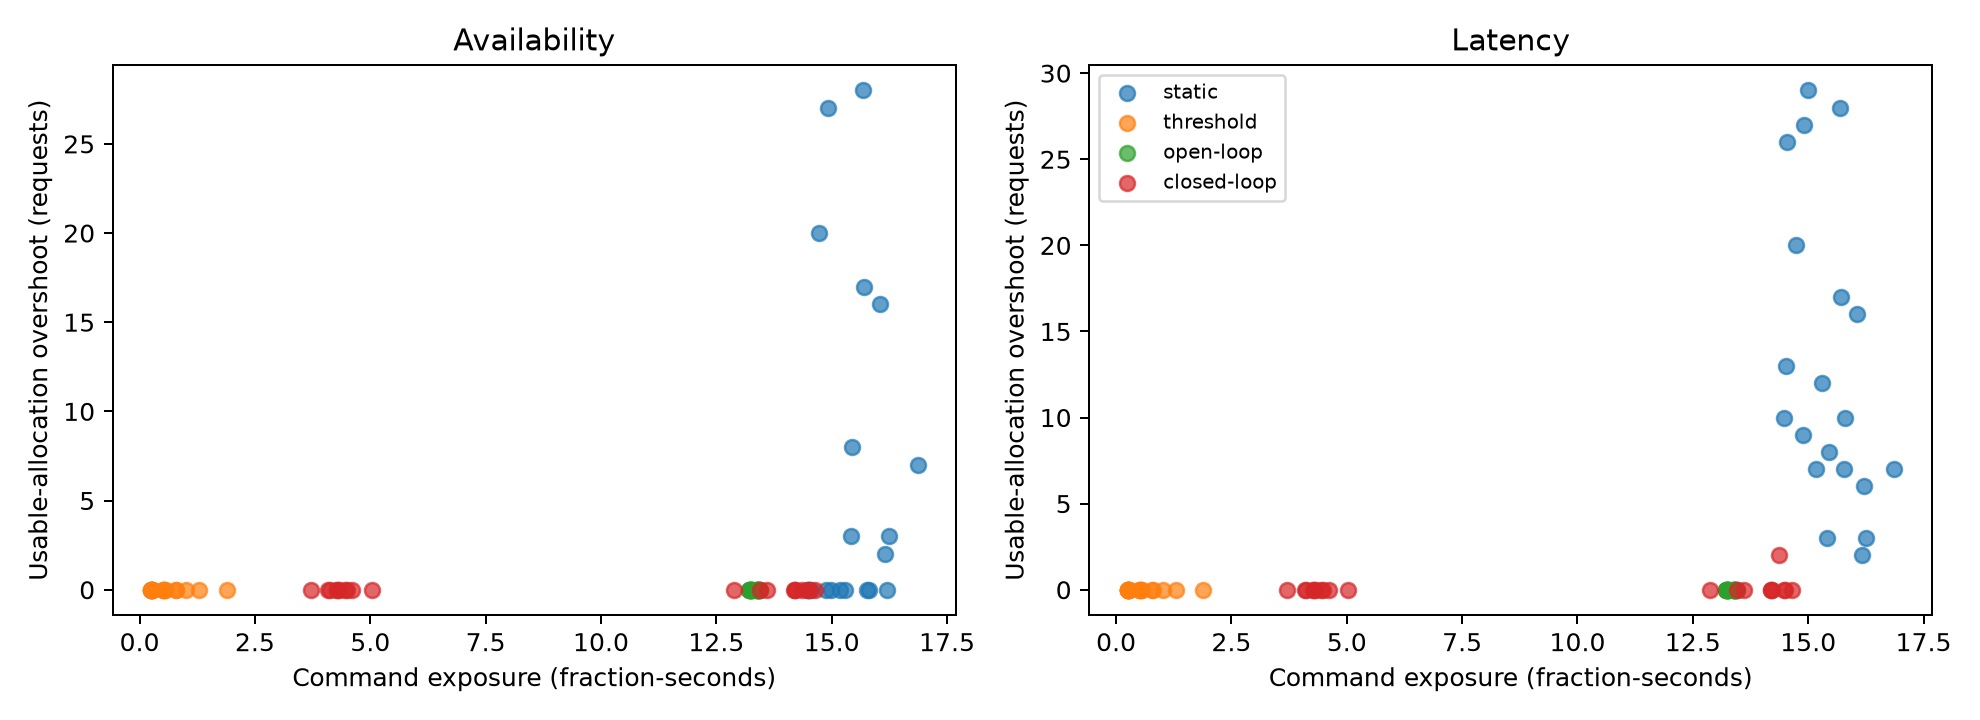
\includegraphics[width=.96\textwidth]{results/curated/study-comparison.png}
\caption{Every verified core run, showing command exposure against usable-allocation overshoot for each SLO ledger.}\label{fig:study}
\end{figure*}

\subsection{Cost per unit of exposure}
Table~\ref{tbl:cost} divides mean bad requests by mean exposure. The ratio is close to the request rate times the pilot cost (about 32 at 32 requests/s and 64 at 64 requests/s) for every policy. A unit of exposure therefore costs about the same number of bad requests under every policy. The policies differ in how much exposure they deliver and in how close they bring the ledger to the guard. The threshold values are less precise because their exposure is very small.

\begin{table}[width=.95\linewidth,cols=5,pos=t]
\caption{Bad requests per fraction-second of exposure (ratio of the means in Table~\ref{tbl:means}, latency ledger).}\label{tbl:cost}
\footnotesize
\begin{tabular*}{\tblwidth}{@{\extracolsep{\fill}}lrrrr@{}}
\toprule
Fault, req/s & Closed & Open & Static & Threshold \\
\midrule
abort, 32 & 31.8 & 31.4 & 30.2 & 36.2 \\
abort, 64 & 65.8 & 63.9 & 63.7 & 69.2 \\
delay, 32 & 31.8 & 31.3 & 32.1 & 29.8 \\
delay, 64 & 64.0 & 63.2 & 64.7 & 59.3 \\
\bottomrule
\end{tabular*}
\end{table}

\subsection{Controlled background attribution (RQ2)}\label{sec:background}
With 0.5\% synthetic organic errors in both cohorts, conservative background credit remained zero in all five attributed runs at 32 requests/s and averaged 25.91 requests at 64. Relative to naive total-loss accounting, the signed point estimate reduced absolute error against the tagged residual reference by 66.78 requests at 32 requests/s (95\% interval [$-68.38$, $-64.97$]) and 134.60 at 64 ([$-138.20$, $-130.99$]). The figures are identical for both ledgers because synthetic organic failures are availability failures and therefore also latency-bad. The better estimate did not lead to more exposure: attributed-minus-total exposure differences were $-0.17$ ([$-0.55$, 0.09]) and $-0.13$ ([$-0.36$, 0.10]) fraction-seconds, and both intervals include zero.

\subsection{Safety mechanism measurements}
Separate integration checks on the same cluster measured the safety mechanisms directly. With a 100\% fault, all 20 treatment requests failed (abort) or were delayed (delay) while all 20 control requests were healthy, confirming treatment-only routing. API cleanup completed in 0.54\,s (abort) and 0.41\,s (delay). When renewal stopped, the unrenewed fault expired after 3.9\,s. After the controller was killed with SIGKILL during injection, the watchdog removed the fault within 7.0\,s, inside the 15\,s reserve window. A run declared with a contaminated control was refused at admission and no fault was applied. These are single checks, not repeated measurements.

\IfFileExists{results/curated/followup-results.tex}{% Generated prose for the post-result budget-paced follow-up (results/raw/followup-paced-v1).
% The table is produced by: python -m cc_cep.followup table --directory results/raw/followup-paced-v1
\subsection{Budget-paced follow-up (post-result)}\label{sec:followup}
After the main study we ran the paced policy of Table~\ref{tbl:policies} in 20 further runs: both fault types at both request rates, using the five v7 block seeds and the frozen v7 runtime. All 20 runs passed evidence verification and replay, giving 128 of 128 planned comparisons with v7 runs. The paced runs were collected about a week after v7 and paired by block ID only, so Table~\ref{tbl:followup} is a descriptive, time-separated comparison and is not pooled with the main study.

The paced policy spent 98--100\% of the usable allocation in every condition, compared with 29--30\% (aborts) and 93--94\% (delays) for the closed-loop policy. Abort exposure rose from 4.46 to 15.41 fraction-seconds at 32 requests/s and from 4.21 to 15.09 at 64 requests/s. Delay exposure rose by 0.98 and 0.76 fraction-seconds, and paced exposure exceeded open-loop exposure by 1.6--2.0 fraction-seconds in all four conditions. Paced exposure was within 0.62 fraction-seconds of static injection, and all four paced-minus-static intervals include zero. Bad requests per fraction-second stayed at about 30--34 at 32 requests/s and 62--66 at 64 requests/s, matching Table~\ref{tbl:cost}, so the extra exposure cost the expected number of bad requests.

The gain came with a small loss of safety margin. Nine of the 20 runs exceeded the usable guard by 1--4 requests, and seven of those were ended early by the common allocation safety guard; the other 13 ran the full window. Mean guard overshoot was 0.8--1.6 requests, compared with 4.6--21.6 for static injection (paired reductions of 3.6--20.0 requests) and almost zero for the closed-loop policy. The 675- and 1,350-request reserves absorbed every overshoot: the largest total was 964 of a 2,310-request allocation. Pacing against the remaining allocation therefore removes the burn-gate under-use. However, it moves the policy close to the guard, and its residual overshoot comes from guard trips once the remaining allocation is nearly spent. A randomized study that runs paced and closed-loop control in the same blocks is still needed before claiming the gain causally.

\begin{table*}[width=\textwidth,cols=7,pos=t]
\caption{Budget-paced follow-up over five blocks. Guard overshoot is in requests and exposure in fraction-seconds, on the latency ledger (an abort counts against both ledgers, so abort values are the same for availability). Means for paced runs, and paced minus v7 differences with 95\% block-bootstrap intervals. The pairing is time-separated, not jointly randomized.}\label{tbl:followup}
\footnotesize
\begin{tabular*}{\tblwidth}{@{\extracolsep{\fill}}llrrrll@{}}
\toprule
Fault & Req/s & Guard overshoot & Exposure & Usable spent & $\Delta$ exposure vs.\ closed-loop & $\Delta$ exposure vs.\ open-loop \\
\midrule
abort & 32 & 1.0 & 15.41 & 98\% & $10.95$ [$10.47$, $11.39$] & $2.00$ [$1.35$, $2.64$] \\
abort & 64 & 1.6 & 15.09 & 100\% & $10.88$ [$10.60$, $11.05$] & $1.69$ [$1.35$, $2.03$] \\
delay & 32 & 1.0 & 15.03 & 99\% & $0.98$ [$0.06$, $1.59$] & $1.80$ [$1.15$, $2.35$] \\
delay & 64 & 0.8 & 14.81 & 99\% & $0.76$ [$0.13$, $1.49$] & $1.56$ [$1.30$, $1.87$] \\
\bottomrule
\end{tabular*}
\end{table*}

}{}

\subsection{Reproducibility}
The portable archive retains all 111 attempts with their source and configuration snapshots, and every selected ledger reconciles with raw client outcomes. An independent extraction on 9 November verified all 173 internal manifests, replayed all 110 selected runs and regenerated the seven analysis outputs byte for byte.

\FloatBarrier

%% ===========================================================================
\section{Discussion}\label{sec:discussion}
%% ===========================================================================

\subsection{Why the feedback controller under-used its allocation}
The closed-loop policy spent about 30\% of its usable allocation in abort runs (142 of 480 and 277 of 960 bad requests) but over 90\% in delay runs (447 of 480 and 899 of 960). Its traces explain the difference. The policy halves intensity when short and long burn exceed 2 and increases it only when burn is below 1. Burn is measured relative to the SLO's allowed bad fraction $q_j$, so for aborts on the 99\% availability SLO it equals 100 times the fault fraction. Abort intensity was therefore confined to roughly 0.5--2\% (mean 1.4--1.5\%) regardless of how much allocation remained. For delays only the 95\% latency SLO burns, at 20 times the fault fraction, so intensity rose to 5\% and stayed there. These SRE burn thresholds are designed to detect unplanned organic consumption, but a chaos experiment is meant to burn budget, so applying them unchanged makes the controller conservative in proportion to how strict the SLO is. The budget-paced follow-up replaces burn with pace relative to the remaining allocation. It was designed after seeing these results, so it is evaluated separately and not pooled. Section~\ref{sec:followup} shows that it spends almost the whole usable allocation, at the cost of small guard trips.

\subsection{What the comparisons can and cannot show}
Some differences follow from the design. The usable headroom was set to half of what static injection at 10\% would consume, so static injection always reaches the guard and its overshoot measures the guard's reaction lag. The threshold policy stops on the first abort interval, so it only gives a lower bound on exposure. In the background ablation, naive total accounting includes the injected organic errors by construction, so the improvement mostly confirms the arithmetic of control subtraction under an ideal independent background. Finally, the two SLOs never constrained the controller together: aborts make both ledgers identical and delays leave availability untouched, so dual-SLO interaction (part of RQ4) remains untested. Overall, feedback control traded exposure for safety, and a well-calibrated open-loop rate was competitive whenever its pilot cost matched the workload.

\subsection{Threats to validity}
Shared-node and transport interference can affect control traffic. Healthy controls and route targeting suggest that the cohorts were isolated, but they cannot prove that there was no interference. Synthetic independent errors are simpler than correlated incidents; confidence-sequence background credit is conditional on that model. Observations are grouped at client-file ingestion boundaries rather than a distributed event-time watermark. Rare-event SLOs, baseline drift, cleanup latency and API readback can all distort short-run accounting. Calibration and pilot fitting can bias comparisons, so their parameters and seeds were frozen before final collection. The benchmark has one synchronous dependency and cannot establish external validity for Online Boutique, infrastructure faults such as pod or node failure, or production services. Load passes through \texttt{kubectl port-forward}, which limited the tested rates. A host-local controller lock does not replace a validated distributed leadership protocol, and the watchdog runs on the same host as the controller. Cluster ablations that remove one SLO or deliberately delay telemetry were not included; unit checks do not replace those experiments. The paced follow-up is compared with runs collected a week earlier, so drift between dates is a threat. The Budget Oracle only summarizes past runs; we have not validated it as an optimizer. Our literature checks found close prior art and were not exhaustive, so we claim only a scoped empirical contribution.

\subsection{Professional, ethical, legal and operational considerations}
\textit{Safety.} Chaos experiments deliberately degrade a service. We limited blast radius to one namespace marked disposable, one route and one dependency, capped intensity at 10\%, made every fault expire after 6\,s unless renewed, and kept an emergency stop and an independent watchdog. In production the same controls would need staffed hours, on-call awareness and predefined abort criteria.

\textit{Security.} The deployment defines a namespaced Role that can only read and patch the named VirtualService and ConfigMap, disables service-account token mounting in workload pods, blocks privilege escalation, and binds port-forwards to localhost. However, the host controller in this study used the local kind administrator kubeconfig, so least privilege was declared but not enforced; a production deployment should run the controller under the restricted service account. Credentials and kubeconfigs are excluded from the repository and evidence archives.

\textit{Privacy.} All traffic was synthetic, and raw logs contain only cohort tags, outcome classes and timestamps. Production request logs can contain personal data, so a real deployment should log only aggregated counts or pseudonymous identifiers and apply a retention limit.

\textit{Legal and contractual.} An internal SLO is usually stricter than a contractual SLA. An experiment allocation must stay inside the internal budget so that deliberate failures never cause SLA breaches, service credits or penalties. Users cannot practically give informed consent to production experiments, so harm must be minimized by small allocations, canary cohorts and immediate stopping.

\textit{Regulatory and governance.} Regulated sectors such as finance and healthcare typically require approved change management and auditable records for deliberate production changes. Our append-only event log, sealed evidence and frozen configuration provide that audit trail, but organizational approval would still be required.

\textit{Research ethics and integrity.} We report mixed and negative results, keep every failed attempt and retry, separate post-result changes from the frozen study, and avoid novelty claims that the literature review cannot support.

\textit{Cost and energy.} The study used one laptop and no cloud resources, so the monetary cost was zero. Energy use was not measured, and roughly 20 hours of continuous cluster operation is a real, if modest, cost.

%% ===========================================================================
\section{Conclusion}\label{sec:conclusion}
%% ===========================================================================
We built and evaluated an SLO-aware chaos engineering controller on Kubernetes and Istio that accounts availability and latency budgets separately in request counts, estimates experiment-caused loss against a matched control, and selects a fault percentage under shared safety guards. The 110-run cluster study shows that the accounting produces no false consumption on healthy traffic and that no policy exceeded its allocation. Feedback control removed the guard overshoot of static injection but delivered less exposure, especially for aborts, where calibrated open-loop injection remained competitive. Trace analysis showed that absolute burn-rate gates caused this, because they cap abort intensity near 2\% under a 99\% SLO. A budget-paced variant, tested in a separate 20-run follow-up, removed that under-use: it delivered close to static exposure with 0.8--1.6 requests of mean guard overshoot, compared with 4.6--21.6 for static injection. Matched estimates improved attribution accuracy under synthetic independent background errors without a clear exposure gain. Future work should repeat the paced policy inside a randomized study, add pod and node failures, run the controller under its restricted service account on a multi-node cluster, and test correlated backgrounds and richer applications such as Online Boutique.

%% Loading bibliography style file
%\bibliographystyle{model1-num-names}
% Loading bibliography database
\bibliography{cas-refs}
\bibliographystyle{cas-model2-names}

\end{document}
